\documentclass[12pt]{article}
\usepackage[margin=1in]{geometry}                % See geometry.pdf to learn the layout options. There are lots.
\geometry{letterpaper}                   % ... or a4paper or a5paper or ... 
\pagestyle{plain} 			    % numbers at bottom of page on page 2+
%\geometry{landscape}                % Activate for for rotated page geometry
\usepackage[parfill]{parskip}    % Activate to begin paragraphs with an empty line rather than an indent
\usepackage{graphicx}
\usepackage{amsmath}
\usepackage{xcolor}
\usepackage{amssymb}
\usepackage{caption}
\usepackage{bm}

\usepackage{gensymb} % for \degree

\usepackage{enumitem} % for enumerate modifications

\usepackage{bbm}

\usepackage{calc}
\usepackage{lipsum}
\makeatletter
\newcommand{\tocfill}{\cleaders\hbox{$\m@th \mkern\@dotsep mu . \mkern\@dotsep mu$}\hfill}
\makeatother
\newcommand{\abbrlabel}[1]{\makebox[4.5cm][l]{\textbf{#1}\ \tocfill}}
\newenvironment{abbreviations}{\begin{list}{}{\renewcommand{\makelabel}{\abbrlabel}%
        \setlength{\labelwidth}{4.5cm}\setlength{\leftmargin}{\labelwidth+\labelsep}%
                                              \setlength{\itemsep}{0pt}}}{\end{list}}                                     


\usepackage{outlines}
\usepackage{enumitem}
\setenumerate[1]{label=\arabic*)} % These are for adjusting the outline letterings 
\setenumerate[2]{label=-}
\setenumerate[3]{label=\roman*.}
\setenumerate[4]{label=\alph*.}

\captionsetup{font=footnotesize}
\usepackage[utf8]{inputenc}

\title{Testbed for Detection and Attribution Methods}
\author{Nathan Lenssen}
\date{December 2017}
\newcommand{\Prob}{\ensuremath{\mathbb{P}}}
\newcommand{\E}{\ensuremath{\mathbb{E}}}
\newcommand{\V}{\ensuremath{\text{Var}}}
\newcommand{\C}{\ensuremath{\text{Cov}}}
\newcommand{\insitu}{\emph{in situ }}

% shortcut for bold
\def\*#1{\bm{#1}}
\def\C{\textbf{\text{C}}}


\begin{document}
\maketitle

\subsection{Description of MATLAB Files in finalCode}
\begin{itemize}
\item \texttt{fullProcedure.m} is a master function that runs the generation procedure, has the option to plot, and saves the relevant output. It takes no more than 30 seconds on my laptop at the current settings.

\item \texttt{parameterList.m} User-set parameters for the Detection and Attribution testbed generation matlab program. Generally the only .m file that should be edited for basic use of the testbed.

\item \texttt{generateSimulation.m} is a script that handles the entire simulation. It returns all of the objects of interest as laid out in Section 0.3, plus a few bonus objects used in plotting. It depends on a few user functions to handle the spatial covariances. It currently needs major attention with respect to the relative scales of $\*x^*$,  $\*y^*$, $\*\nu$, and $\*\eta$.

\item \texttt{makePlots.m} Creates all of the plots found in this report if plotting is turned on when \texttt{fullProcedure.m} is run. Will be expanded as the project progresses.

\item \texttt{writeOutput.m} Saves the relevant objects to disk. Will eventually save as netCDF to facilitate sharing between programming languages.

\item \texttt{generateMatern.m} is an evaluation of the Mat\'ern radial basis function as done in \texttt{fields}. It is used to generate the spatial covariance of the forced responses.

\item \texttt{generateRecBasis.m} returns the eigenvectors and eigenvalues of an exponential covariance matrix on a $[0,1] \times [0,1]$ grid for a given scale parameter.

\item \texttt{generateCovExact.m} returns various covariance objects of the modified exponential to be used as the internal climate variability $\C$. The modification is an in Hannart 2016 in which the eigenvalues of a exponential covariance matrix are modified by multiplicative random factors.

\item \texttt{runLocal.sh} runs the testbed on a local machine. Note that matlab must be correctly added to the PATH variable

\item \texttt{runHabanero.sh} runs the testbed on the Habanero cluster. Useful for users that do not have local access to MATLAB
\end{itemize} 


\subsection{Model and parameters of interest}
Following equation (3) \cite{hannart16}, we work with the classical problem for detection and attribution where $\*y$ is the observed spatial climate response, $\* x_j$ with $j = 1, \dots, J$ are the externally forced signals, and $\*\Sigma$ is the internal climate variability.
\begin{align}
\*y &= \*x^* \*\beta + \*\nu \qquad \*\nu_j \stackrel{iid}{\sim} \mathcal{N}_n(0, \*\Sigma) \nonumber\\
\* x &= \*x^* + \, \*\eta \qquad \,\, \*\eta_j \stackrel{iid}{\sim}  \mathcal{N}_n(0, \*\Sigma/m) 
\end{align}

To make explicit that the fingerprints we are regressing in the EIV model above are ensemble means, we let $\*{\bar x}$ be the matrix of ensemble means for the forced climate responses and rewrite. Letting $\C$ represent the internal climate variability we define 
\begin{align} \label{eq:hForm}
\*y &= \*x^* \*\beta + \*\nu \qquad \*\nu_j \stackrel{iid}{\sim}  \mathcal{N}_n(0, \C) \nonumber\\
\*{\bar x} &= \* x^* + \, \*\eta \qquad \,\, \*\eta_j \stackrel{iid}{\sim}  \mathcal{N}_n(0, \C/m).
\end{align}
Adding in the notation from [Smith et al., 20xx] where we include a superscript $\*x_j^{(\ell)}$ with $\ell = 1, \dots , L$ to represent ensemble members for a given forcing, we unpack to see the ensemble behavior of the climate variability in the forced responses
\begin{align}
\*y &= \*x^* \*\beta + \*\nu \qquad \qquad \:\:\:\, \*\nu_j \stackrel{iid}{\sim}  \mathcal{N}_n(0, \C) \nonumber\\
\*{\bar x} &= \* x^* + \, \frac{1}{m}  \sum_{\ell=1}^L \*\nu^{(\ell)} \quad \, \,\,  \*\nu_j \stackrel{iid}{\sim}  \mathcal{N}_n(0, \C) \\
&= \* x^* + \, \*\eta \qquad \qquad \quad \,\, \*\eta_j \stackrel{iid}{\sim}  \mathcal{N}_n(0, \C/L) \nonumber
\end{align}
Given the formulation presented in equation \ref{eq:hForm}, the primary goals of inference the $\*\beta$ and $\C$ parameters. In the development of a testbed, we need to simulate all of these objects (see Section 0.4 for full list) and organize in an intuitive and efficient way.

\textcolor{red}{\emph{This notation is still under development and clearly a poor middle ground in places. Possibly discuss today the best way to merge the notation of Alexis, Aur\'elien, Philippe, et al.\ with the notation of Richard, Matthias, Dorit et al. for the final code and documentation.}}

\subsection{Assumptions for Simulation}
Using the framework proposed by Alexis in Section 4a of \cite{hannart16} as a starting point, we create a preliminary testbed with the following assumptions:
\begin{enumerate}[label={(\Roman*)}]
\item We assume that the climate variability in the observed climate signal $\*\nu$ is proportional to the climate variability in the ensemble mean of the forced signal $\*\eta$ through the ensemble size. This is different from  The $L^{-1}$ scaling in the covariance of $\*\eta$ is assuming the fingerprints used are ensemble means. A clear and relatively simple extension is to incorporate the $\alpha$ and $\gamma$ covariance scaling factors that are introduced in [Smith et al., 20xx]
\item We assume that the internal climate variability $\C$ has a form as in \cite{hannart16}. The generative process is modifying the eigenvalues of a exponential covariance matrix by multiplicative random factors. This procedure is a computationally efficient way to generate a covariance structure that is non-isotropic.
\item We assume that the unobserved regressors $\*x^*$, with columns $\*x^*_j$ a single forced fingerprint, have spatial covariance according to the Mat\'ern $\*\Sigma_{x_j}$. This covariance structure is not representative of the noise on the simulated $\*x_j^{(\ell)}$ which is represented in Equation \ref{eq:hForm}, but rather the underlying structure of the true forced climate responses $\*x^*_j$. Furthermore, we can specify a different spatial correlation for each simulated forced response. We also assume that the columns of $\*x^*$ are independent.

Note that this is different than the forced responses in \cite{hannart16} where they were taken to be spatially independent, but correlated across forcings. In conversation with Alexis, we decided to proceed with generating our forced responses with spatial correlation and forcing independence for now.

\item \textcolor{red}{Further work is needed thinking about to control the relative scales of the signal from the forcing responses and the noise from the internal climate variability. This could be handled in the simulation by the addition of the covariance scaling parameters suggested by Richard.}
\end{enumerate}

\subsection{Applicability to Smith et al.\ 20xx and KHS 2017}
The model for $\*y$ in \cite{khs17} is given in equation (8) of Smith et al.\ 20xx as
\begin{equation}
\*y | \*x_1, \dots \*x_J, \*\beta, \C \quad \sim \quad \mathcal{N}_n \left [ \sum_{j=1}^J \*x_j \beta_j ,\C \right ] 
\end{equation}

The extension proposed in Smith et al.\ 20xx is adding a scaling factor $\alpha$ to control the relationship between the noise in the control run and forced run simulations.
\begin{equation}
\*y | \*x_1, \dots \*x_J, \*\beta, \C, \alpha \quad \sim \quad \mathcal{N}_n \left [ \sum_{j=1}^J \*x_j \beta_j , \alpha^{-1}\C \right ] 
\end{equation}

The model error for a single forcing $j$ for a single realization $\ell$ allowing for forcing specific scaling factors $\gamma_j$ is
\begin{equation}
\*x_j^{(\ell)} | \*x_j, \C, \gamma \quad \sim \quad \mathcal{N}_n\left [  \*x_j, \gamma_j^{-1}\C  \right ], \; \ell = 1, \dots, L, \;j= 1, \dots, J.
\end{equation}
The Bayesian formulations are particularly useful in the context of a testbed simulation as they directly prescribe a procedure for generating data. 

The major assumptions made in Smith et al.\ 20xx are
\begin{enumerate}[label={(\Roman*)}]
\item We no longer require as strict of an assumption as (I) in the Hannart formulation. We allow scaling between the various models through $\alpha$ and between the various forcing scenarios through $\gamma$. 
\item The dimension reduction of the climate variability $\C$ is handled by informative priors
\item Additional flexibility in handling ensembles of $\*y$ by allowing another variance term $\*W$ to model the behavior of the observational noise.
\end{enumerate}


\subsection{Objects of Interest}
Relevant sizes:
\begin{itemize}
\item $n$ the number of observations
\item $r$ the number of control runs used in the estimation of $\C$ ($r \ll n$)
\item $k$ the number of fingerprints/PCs/eigenvectors to be used in the analysis ($k \leq r$)
\item $L$ the size of the ensemble for each forcing (will eventually be $L_j$)
\item $J$ the number of externally forced signals (regressors)
\end{itemize}
Objects that simulate the real problem we are facing:
\begin{itemize}
\item $\*y$ the observed climate change field $[n \times 1]$
\item $\* {\bar x}$ the model-mean fingerprints from the $p$ forcing response runs $[n \times J]$
\item $\* x$ the $m$ ensemble member fingerprints from the $p$ forcing response runs $[n \times (L\cdot J)]$
\item $\*\varepsilon = (\varepsilon_1, \dots, \varepsilon_r)$, the control runs used to estimate $\C$ $[n \times r]$
\end{itemize}
Underlying objects from the simulation that we return to evaluate our performance:
\begin{itemize}
\item $\*y^*$  the `true' climate change pattern $[n \times 1]$
\item $\*x^*$  The `true' fingerprints for each forcing $[n \times J]$
\item $\*\Sigma_x$ the spatial covariance used to generate the pattern of the $\*x^*$. Note that this covariance is not necessarily equal for all patterns. $[n \times n \times J]$
\item $\*\beta$  the `true' coefficients $[J \times 1]$
\item $\C$  the `true' internal variability $[n \times n]$
\end{itemize}

Objects that we are evaluating our inference of:
\begin{itemize}
\item $\*{\hat\beta}$ the coefficients of attribution $[J \times 1]$
\item $\hat \C$ the internal climate variability $[n \times n]$
\end{itemize}



\clearpage
\subsection{Initial Simulation Outline}

\begin{outline}[enumerate]
In this initial simulation we set the number of observations $n = 2500 = 50^2$ on the unit square, the number of forced signals $J =2$ with $\*\beta = (\beta_1, \beta_2) = (1,1)$. The rest of the simulation procedure is as follows:
\1 Generate the internal variability $\C$ with the modified eigenvalues method
\2 We specify the scale of the exponential kernel and the magnitude of the random factors used to modify the eigenvalues
\2 Additionally, the climate variability $\C$ is whitened according to the parameter $\rho$
\2 Various visualizations of the resulting $\C$ can be seen in Figures \ref{fig:corr1} and \ref{fig:corr2}.
\1 Calculate $\*\Sigma_{x_j}$ from the Mat\'ern family for each of the forced responses
\2 To demonstrate the capabilities of the testbed, we set one forcing very smooth and long range and the other forcing rough and short range.
\1 Generate the true forcing responses $\*x^*_j$ using $\*\Sigma_{x_j}$ for the forcing-specific correlation.
\2 The fields for $\*x^*_1$ and $\*x^*_2$ can be seen in the top left panel of Figures \ref{fig:xfield1} and \ref{fig:xfield2}.
\1 Simulate the observed forcing responses $\*x^{(\ell)}_j = \*x^*_j + \*\nu$ for each forcing $j$ and for each ensemble member $\ell$. 
\2 We calculate the ensemble means of the forcing responses $\*{\bar x}_j = \frac{1}{L}\sum_{\ell =1}^L \*x^{(\ell)}_j$
\2 The ensemble means are plotted in the top right of Figures \ref{fig:xfield1} and \ref{fig:xfield2}.
\2 Ensemble members are plotted in the bottom four plots of Figures \ref{fig:xfield1} and \ref{fig:xfield2}.
\1 Simulate the control runs from $\mathcal{N}(0,\C)$ 
\2 We currently simulate 300 members so that the sensitivity of methods to the size of the control run sample can be easily tested without rerunning the testbed simulation.
\1 Calculate the true climate response according to $\*y^* = \*x^* \*\beta $ 
\2 Shown in the top left of Figure \ref{fig:yfield}
\1 Simulate a climate response $\*y = \*x^* \*\beta + \*\nu$
\2 Shown in the top right of Figure \ref{fig:yfield}

\end{outline}

\clearpage
\begin{figure}[htbp]
\begin{center}
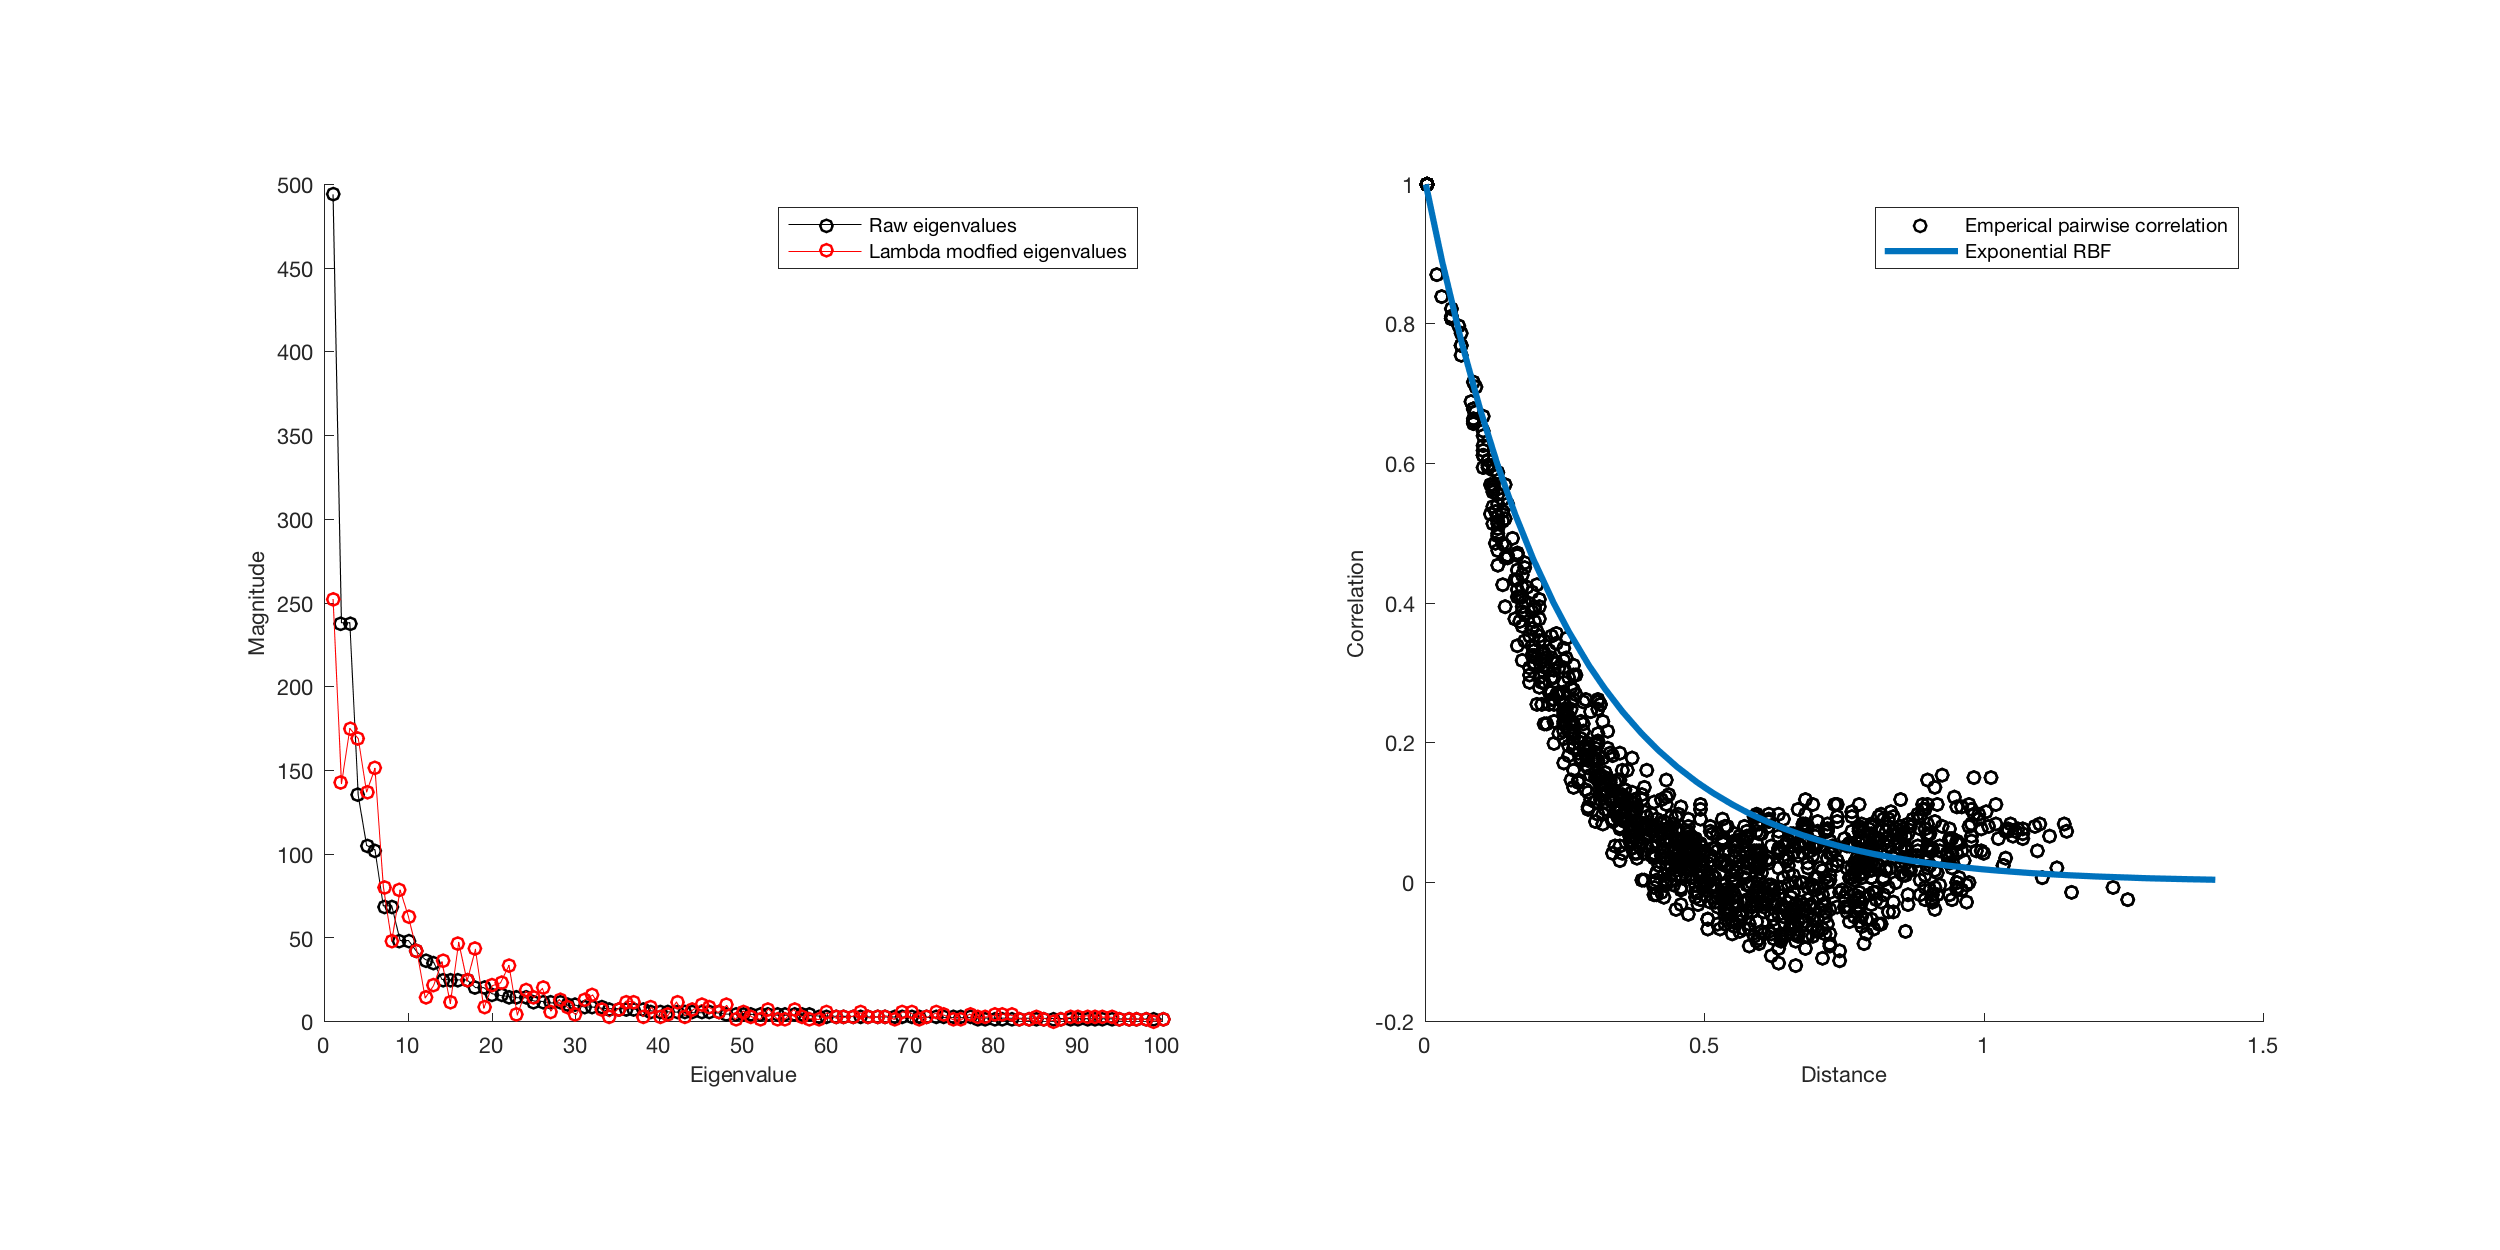
\includegraphics[width=0.8\textwidth]{figures/checkExp.png}
\caption{\textbf{Left:} Visualization of the modification to the eigenvalues of the exponential covariance matrix for the construction of the climate variability $\C$ \textbf{Right:} Comparing the observed pairwise correlations in $\C$ with the exponential (without modified eigenvalues) as in Figure 3(c) of Hannart 2016.}
\label{fig:corr1}
\end{center}
\end{figure}

\begin{figure}[htbp]
\begin{center}
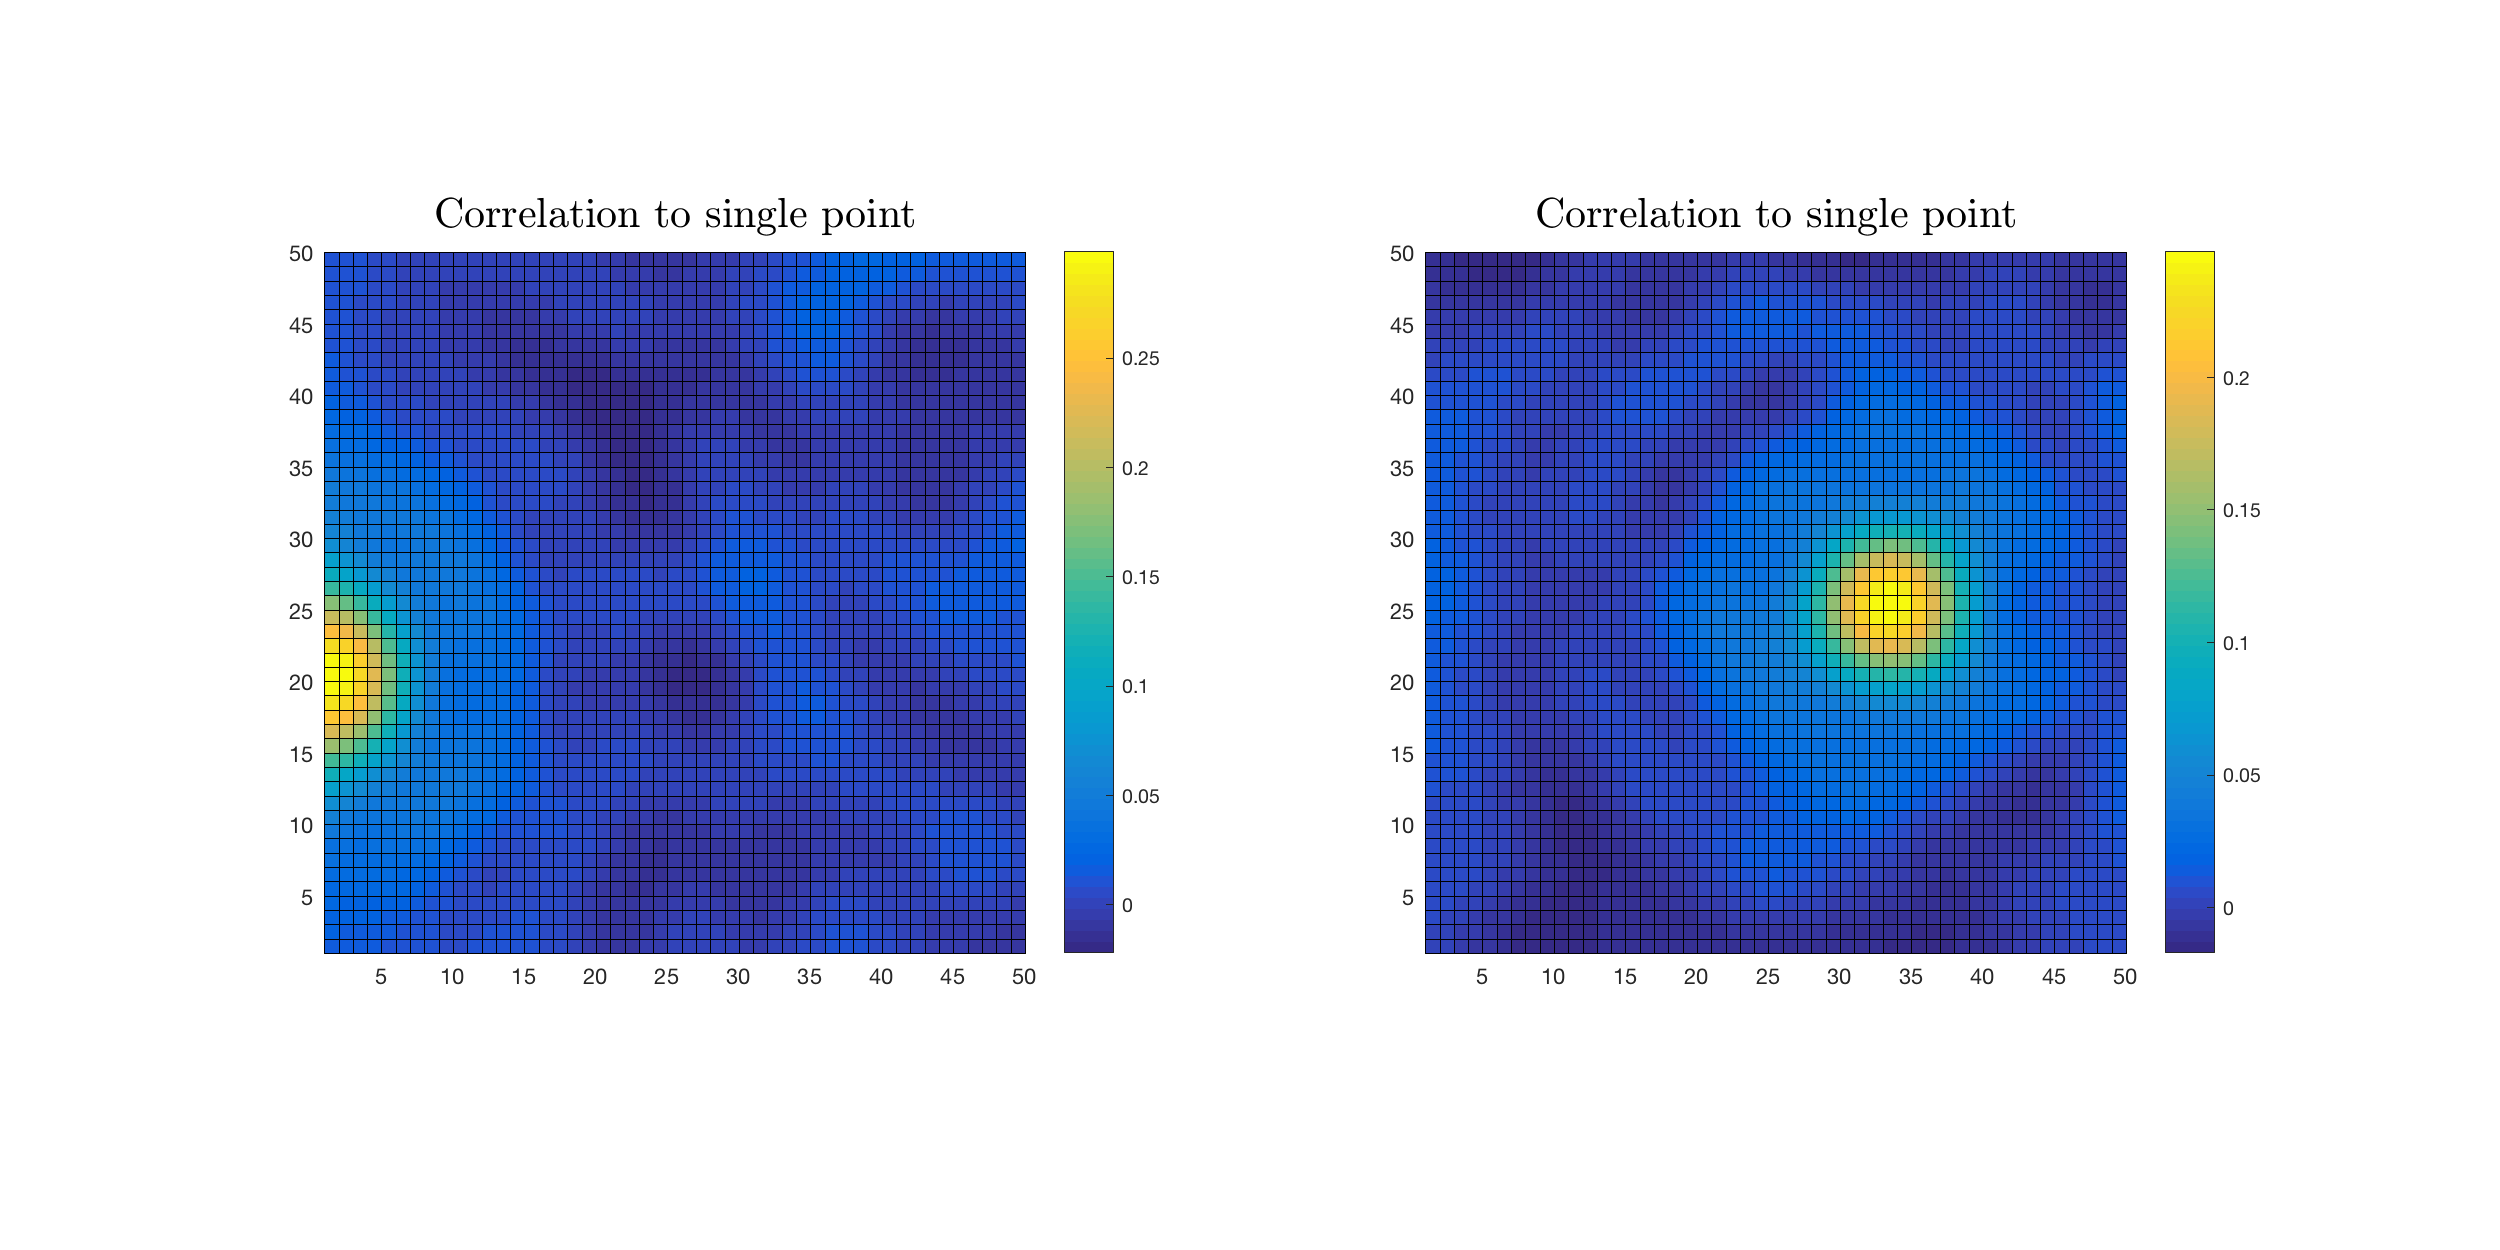
\includegraphics[width=0.85\textwidth]{figures/ptCorrelation.png}
\caption{Two single points correlation matrices according to the climate internal varability $\C$. We are viewing the same covariance matrix from two different points as in Figure 3(d) of Hannart 2016.}
\label{fig:corr2}
\end{center}
\end{figure}

\begin{figure}[htbp]
\begin{center}
\includegraphics[width=0.9\textwidth]{figures/xgeneration1.png}
\caption{The relationship between the underlying true $\*x^*_1$ and the observed ensemble mean fingerprint $ \*{\bar x_1}$. Individual ensemble members are shown in the bottom four plots.}
\label{fig:xfield1}
\end{center}
\end{figure}

\begin{figure}[htbp]
\begin{center}
\includegraphics[width=0.9\textwidth]{figures/xgeneration2.png}
\caption{The relationship between the underlying true $\*x^*_2$ and the observed ensemble mean fingerprint $ \*{\bar x_2}$.  Individual ensemble members are shown in the bottom four plots.}
\label{fig:xfield2}
\end{center}
\end{figure}


\begin{figure}[htbp]
\begin{center}
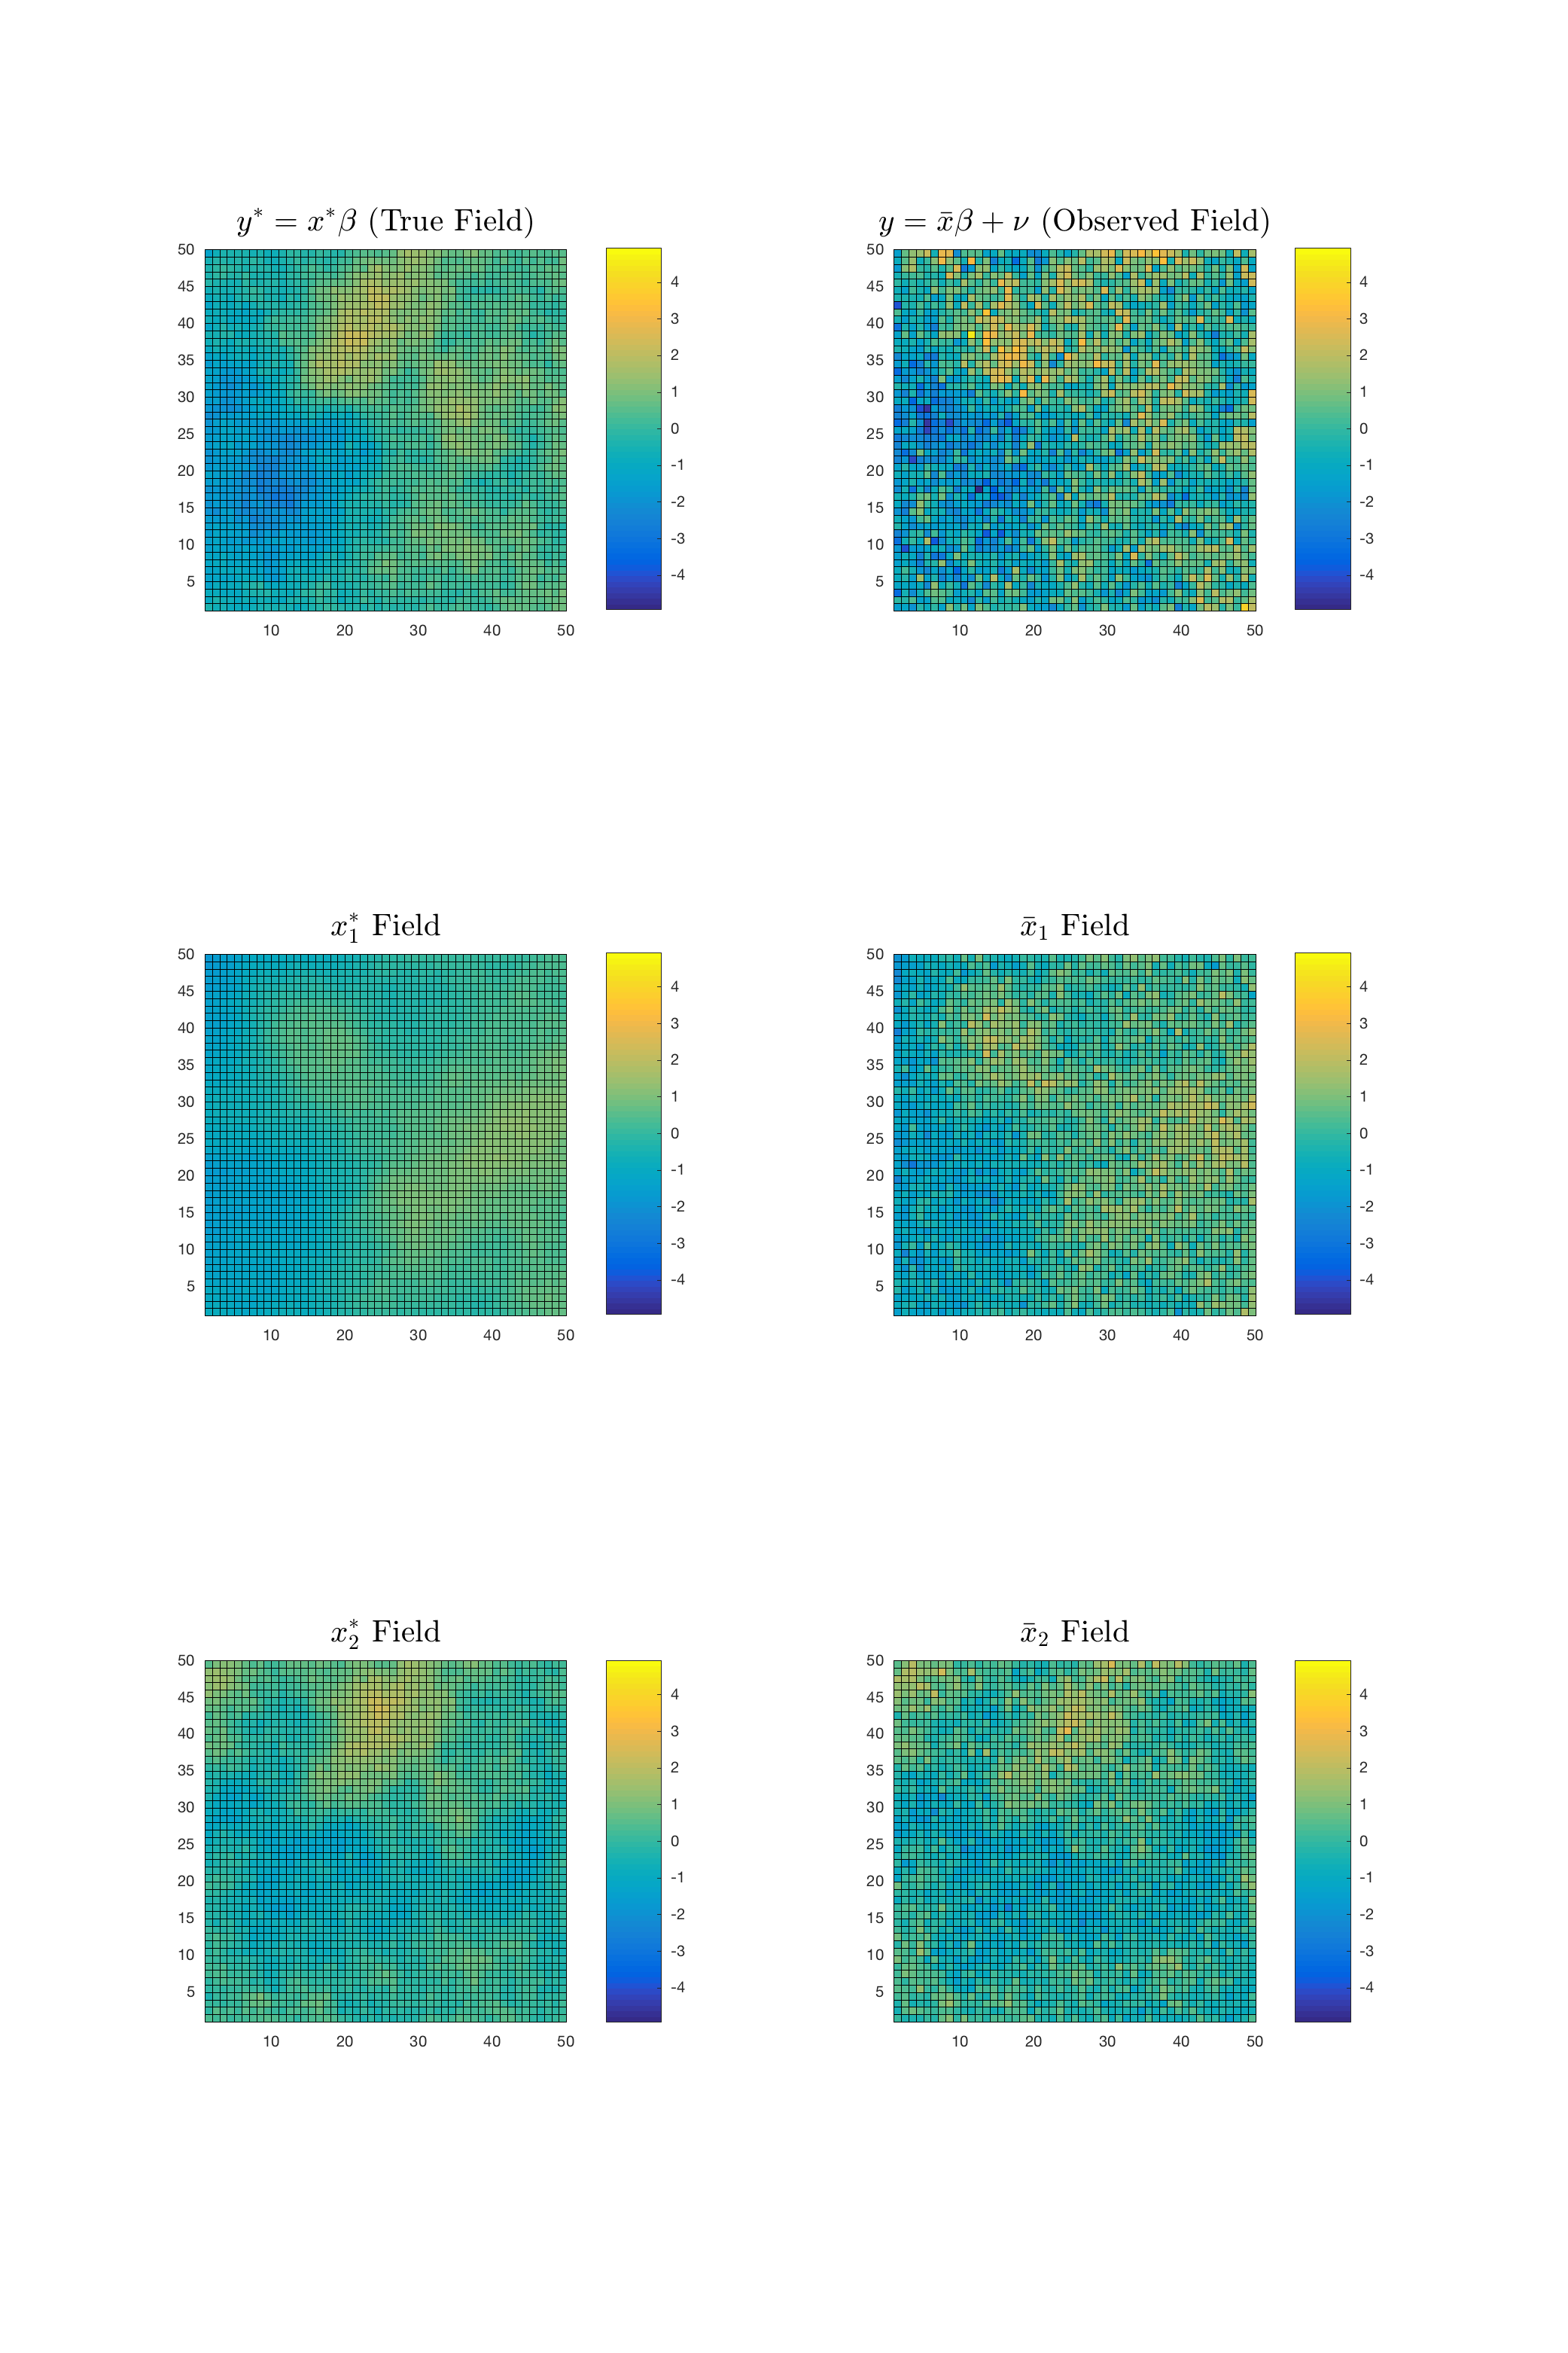
\includegraphics[width=0.9\textwidth]{figures/yprogression.png}
\caption{The progression of the $\*y$ object as it is built. The true latent objects are in the left column and the observed objects are on the right. Since $\*\beta = (1,1)$, the top row is the sum of the bottom two rows.}
\label{fig:yfield}
\end{center}
\end{figure}


\newpage
\bibliographystyle{apalike}

\bibliography{testbedReferences}

\end{document}